\documentclass{standalone}
\usepackage{tikz}

\begin{document}

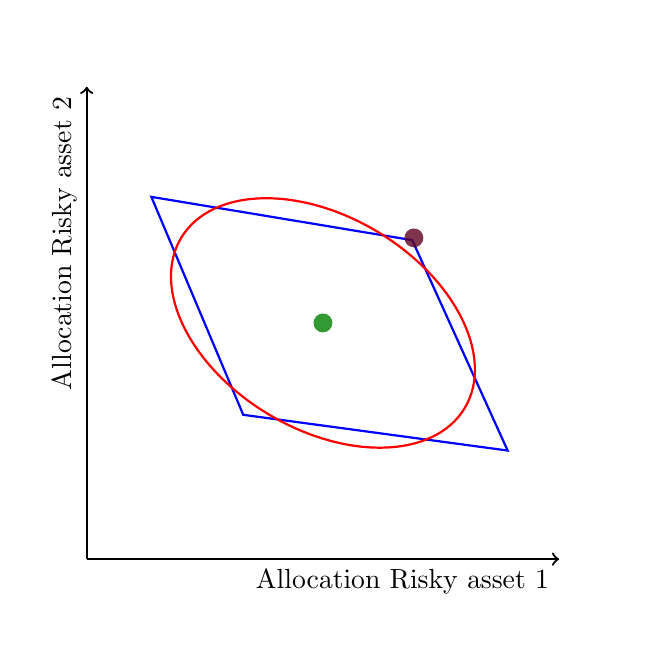
\begin{tikzpicture}[scale=1.5]% Shift diagram to add space
    \useasboundingbox (-0.5, -0.5) rectangle (4.5, 4.5);
    % Invisible bounding box extension
    \draw[opacity=0] (-1, 0) -- (4.5, 0); % Extend x-axis left and right
    \draw[opacity=0] (0, -1) -- (0, 4.5); % Extend y-axis down and up
    % Axes
    \draw[thick, ->] (0, 0) -- (4, 0) node[below left] {Allocation Risky asset 1}; % x-axis
    \draw[thick, ->] (0, 0) -- (0, 4) node[above left, rotate=90] {Allocation Risky asset 2}; % y-axis

    % Blue Parallelogram
    \draw[thick, blue, rotate around={20:(2,2)}] 
        (1.1, 1.5) -- (3.1, 0.45) -- (2.95, 2.4) -- (1., 3.5) -- cycle;
    % lower left, lower right, upper right, upper left
    % Red Ellipse
    \draw[thick, red, rotate around={149:(2,2)}] 
        (2, 2) ellipse (1.4 and 0.9);

    % Green Center Point
    \fill[green!50!black,opacity=0.8] (2, 2) circle (0.08);

    % Green Center Point
    \fill[purple!50!black,opacity=0.8] (2.77, 2.72) circle (0.08);    

\end{tikzpicture}

\end{document}